% We're currently using this project to write the UD Evaluation paper on the evaluation of the reannotation of UD_Turkish-BOUN, which resulted in v2.11. As of Oct 10, this is the up-to-date project.

% LREC-COLING 2024 Example;
% LREC Is now using templates similar to the ACL ones.
\documentclass[10pt, a4paper]{article}

\usepackage[review]{lrec-coling2024} % this is the new style

                 % Use more than one optional parameter in a new commands
%\usepackage[dvipsnames]{xcolor}  % Coloured text etc. now in acmart.cls
\usepackage[colorinlistoftodos,prependcaption,textsize=small]{todonotes}
\usepackage{leipzig}
\usepackage[linguistics]{forest}
\usepackage{gb4e}
\usepackage{epstopdf} 
\RequirePackage{xspace}
\makeglossaries
\usepackage{xargs}   
\usepackage{subcaption}
\newcommandx{\unsure}[2][1=]{\todo[linecolor=red,backgroundcolor=red!25,bordercolor=red,#1]{#2}}
\newcommandx{\change}[2][1=]{\todo[linecolor=blue,backgroundcolor=blue!25,bordercolor=blue,#1]{#2}}
\newcommandx{\feedback}[2][1=]{\todo[linecolor=yellow,backgroundcolor=yellow!25,bordercolor=yellow,#1]{#2}}
\newcommandx{\improvement}[2][1=]{\todo[linecolor=green,backgroundcolor=green!25,bordercolor=green,#1]{#2}}
\newcommandx{\thiswillnotshow}[2][1=]{\todo[disable,#1]{#2}}
\newcommandx{\completedRevision}[2][1=]{\todo[disable,backgroundcolor=red,#1]{#2}}
\newcommandx{\dataSource}[2][1=]{\todo[disable,backgroundcolor=red,#1]{#2}}

%\usepackage{ascii}
\usepackage{hyperref}
 \definecolor{darkblue}{rgb}{0, 0, 0.5}
  \hypersetup{colorlinks=true, citecolor=darkblue, linkcolor=darkblue, urlcolor=darkblue}

\usepackage{tabularx}  % Load the tabularx package
\usepackage{seqsplit}  % Helps to split long text sequence

\usepackage{siunitx}   
\sisetup{input-decimal-markers={.},output-decimal-marker={.},group-separator={.},detect-weight,group-minimum-digits=4,group-digits=integer}
\renewcommand{\ttdefault}{cmtt}


\title{Evaluating the quality of a corpus annotation scheme using pretrained language models}

\name{Author1, Author2, Author3}

\address{Affiliation1, Affiliation2, Affiliation3 \\
         Address1, Address2, Address3 \\
         author1@xxx.yy, author2@zzz.edu, author3@hhh.com\\
         \{author1, author5, author9\}@abc.org\\}

\abstract{
Pretrained language models and large language models are increasingly used to assist in a great variety of natural language tasks.
In this work, we explore their use in evaluating the quality of alternative corpus annotation schemes.
For this purpose, we analyze two alternative annotations of the Turkish BOUN treebank, versions 2.8 and 2.11, in the Universal Dependencies framework using large language models. 
Using a suitable prompt generated using treebank annotations,  large language models are used to recover the surface forms of sentences. 
Based on the idea that the large language models capture the characteristics of the languages, we expect that the better annotation scheme would yield the sentences with higher success. 
The experiments conducted on a subset of the treebank show that the new annotation scheme (2.11) results in a successful recovery percentage of about 2 points higher.
 \\ \newline \Keywords{treebank annotation, large language models, universal dependencies, morphologically rich languages, Turkish } }

\begin{document}
\newcommand{\bounvOLD}{UD Turkish BOUN v2.8}
\newcommand{\bounvNEW}{UD Turkish BOUN v2.11}
\newcommand{\ewt}{UD English EWT}
\newcommand{\conllu}{CoNLL-U}


\maketitleabstract

\section{Introduction}
\label{sec:introduction}

The use of pretrained language models and large language models have led to a paradigm shift in solving several types of natural language processing (NLP) tasks. 
Pretrained language models like BERT~\cite{devlin-etal-2019-bert} and GPT~\cite{brown2020language} build a general model that encodes the characteristics of a language or multiple languages, and enable one to adapt this model to the task at hand. 
Large language models like ChatGPT~\cite{openai2021gpt35} and LLaMA~\cite{touvron2023llama} go a step further. 
They provide models that can be used in different types of tasks in zero- or few-shot settings.

Universal Dependencies (UD)~\cite{de2021universal} project is a framework that provides treebanks in a dependency grammar format~\cite{bauer1979some, debusmann2000introduction, de2019dependency} in more than 100 languages~\citetlanguageresource{nivre-etal-2020-universal}. 
It is commonly used for different purposes in the NLP community, including cross-lingual part-of-speech (POS) tagging~\cite{parvez-chang-2021-evaluating}, semantic parsing~\cite{reddy-etal-2017-universal}, and language identification~\cite{toftrup-etal-2021-reproduction}. 
The UD project aims at unifying the annotations of the treebanks and arriving at consistent annotations by introducing a set of principles, universal tags and their language-specific subcategories related to morphosyntax. 
However, due to the varying characteristics of languages in different language families and the different theoretical frameworks followed by linguists, various approaches have emerged in annotating treebanks. 
Some linguistic phenomena in languages that the mechanisms in the framework cannot easily handle are attempted to be addressed in various ways by utilizing the MISC (miscellaneous) field in the \conllu\ format. 
Even the treebanks of the same language may use different annotation strategies for the same linguistic phenomenon depending on the annotators' linguistic theory and assumptions. 
The annotation differences are typically in token splits, lemmas, part-of-speech tags and morphological features of tokens, and types of dependency relations between tokens. 
In addition to such conflicting annotations, the treebanks include noise at both morphological and syntactic levels.

There are different strategies to assess the quality of annotations in corpora, such as measuring the annotation agreement in a controlled setting or using the corpora in downstream tasks. 
The drawback of these approaches is that either they require a great deal of dedicated time and effort by area experts or  suitable downstream tasks must be identified, which may require resources that are not easily attained for all languages.

In this work, we propose a novel method that makes use of large language models (LLM) in evaluating corpus annotation. 
As an application of the proposed approach, we compare the token-level annotations (specifically lemmas, part-of-speech tags, and morphological features) between the two versions of the Turkish BOUN Treebank in the UD framework, the versions 2.8 and 2.11. 
For each treebank, by feeding the annotations of the tokens in natural language to an LLM via a prompt, we expect the LLM to generate the tokens in order with their correct surface forms.
We then compare the output sentences of both versions to determine which one is closer to the original sentence, which signals that the annotation of that sentence is of higher quality and expressivity than the other one. 
We show that, compared to other strategies, the proposed approach is highly efficient and applicable to any language due to the existence of multilingual LLMs.

The contributions in this work are as follows:
\begin{itemize}
    \item A novel approach to assess the quality of corpus annotation, employing large language models.
    \item The application of the method to dependency treebanks to evaluate treebank annotations using a new strategy.
    \item A detailed analysis of the correctness of the annotations in two versions of a treebank based on several parameters, such as token recovery accuracy and morphological feature importance.
\end{itemize}

The remainder of this paper is organized as follows: Section~\ref{sec:background} provides information about background information necessary to follow this work, Section~\ref{sec:related-work} introduces related work, Section~\ref{sec:method} introduces our proposed method, which is followed by experiments and results in Section~\ref{sec:results}. Finally, we conclude with Section~\ref{sec:conclusions}.

% neden llm, bunu açıklayıp justify ediyoruz. morph rich dillerde assessmentın zorluğu, llmin bu konuda anlamlı olması vs.
% Collaborative

% \begin{enumerate}
    % \item use simpler ML models (for some this should be used: input: features, output: choose the correct one out of ten examples)
    % \item use BERT?
    % \item use DeBERTa?
    % \item T5
%     \item ChatGPT
% \end{enumerate}

% ALT paperi

% ??? UD parseriyla yapilan deneyler?

% \begin{enumerate}
%    \item cumlelerin kategorileri var mi?
%    \item kelimelerin kategorileri var mi?
% \end{enumerate}
\section{Background}
\label{sec:background}


\subsection{Universal Dependencies (UD) and BOUN Treebank}
\label{sec:background:ud}
% Busra
The UD Turkish BOUN treebank comprises 9,761 UD-style annotated sentences from various domains, such as biographical texts, newspaper articles, essays, instructional texts, and more.
These sentences were randomly extracted from the Turkish National Corpus~\cite{aksan2012construction}, encompassing different registers.
Importantly, the BOUN treebank data faithfully captures the unique characteristics of Turkish, which include its relatively free word order and licensing pro-drop in addition to object drop.
For a comprehensive analysis of word order distribution within the BOUN treebank, refer to Table \ref{tab:wordord}.

\begin{table}[h]
    \centering
    \begin{tabular}{|c|S[table-format=4]|S|} \hline 
         \multicolumn{1}{|c|}{\textbf{Order}}&  \multicolumn{1}{c|}{\textbf{Count}}& \multicolumn{1}{c|}{\textbf{\%}}\\ \hline 
         OV&  5744& 37.21\\ \hline 
         SV&  5416& 35.09\\ \hline 
         SOV&  1456& 9.43\\ \hline 
         VS&  1116& 7.23\\ \hline 
         VO&  714& 4.63\\ \hline 
         OVS&  549& 3.56\\ \hline 
         VSO&  165& 1.07\\ \hline 
         SVO&  144& 0.93\\ \hline 
         OSV&  109& 0.71\\ \hline 
 VOS& 23&0.15\\ \hline
    \end{tabular}
    \caption{Word order distribution in the BOUN treebank. \textit{S: Subject, O: Object, V: Verb}}
    \label{tab:wordord}
\end{table}

The older version of the UD Turkish BOUN treebank, v2.8~\cite{turk2022resources}, had undergone a semi-automated annotation process in its inception.
Initially, sentences were parsed and syntactically annotated using~\citeauthor{kanerva2018turku}'s parsing pipeline, while morphological annotations were applied using~\citeauthor{sak2011resources}'s morphological disambiguator.
These annotations were then meticulously reviewed and improved by native Turkish speakers.
It's worth noting that there were no newly introduced annotation practices or deviations from the Universal Dependencies (UD) standards in terms of annotation or lemmatization in this version.

This particular version suffered from notable limitations in terms of abstraction and expressiveness, primarily due to the disparities between the annotation framework of UD and the morphologically rich and highly syncretic nature of the Turkish language.
Additionally, the prevalent use of morphophonologically null morphemes, such as the 0-morpheme copula, and highly productive derivational processes in Turkish contributed to these challenges.

UD, initially developed by speakers of morphologically sparse and highly isolating languages like Indo-European languages, adheres to a rigid and specific approach regarding word structure, derivation, lemma splitting, and null morphemes.
This approach considers derivational processes and affixes to be opaque, based on the observation that in most languages derivational affixes typically precede inflectional ones.
In contrast, languages such as Turkish exhibit a different pattern.
For example, \textit{-ki} which derives pronominals can follow genitive and locative case suffixes which are inflectional and further inflectional material such as the plural suffix can be applied to the stem derived by \textit{-ki} as shown in~\ref{evdekiler}:

\begin{exe}
\label{evdekiler}
    \ex 
    \gll ev -de -ki -ler \\
    home LOCATIVE ki PLURAL \\
    \glt \textit{`{[the ones]} at home}' \\
\end{exe}

Additionally, the UD framework lacks a consistent and unified approach to handling morphophonologically null morphemes.
As a result, languages featuring these morphemes have resorted to diverse strategies for annotation~\cite{marton2013dependency, ravishankar2017universal, dyer2022new}.
These limitations within the UD framework have been recognized, prompting discussions and debates within the UD community~\cite{gerdes2016dependency}.
Some topics like wordhood and word segmentation~\cite{seyoum2018universal} remain subjects of ongoing debate in this context.
In addition, researchers adopt different strategies to mitigate the shortcomings of UD in handling of the morphologically rich languages~\cite{more2016data, vincze2017universal, seyoum2018universal}, function words~\cite{osborne2019status}, and various other language-specific phenomena like case-drop~\cite{sundar-ram-lalitha-devi-2021-dependency-parsing}.

Version 2.11 of the BOUN treebank addresses the challenges related to null morphemes, lemmatization, intertwining derivational and inflectional processes, and syncretism within the Turkish language, all while staying as faithful as possible to the UD framework.
The primary objective behind creating v2.11 is to enhance the representational capabilities and both theoretical and practical accuracy of the BOUN treebank.

To achieve this goal, the entire treebank underwent a meticulous manual reannotation process, conducted by linguists who are native speakers of Turkish with domain expertise.
Throughout this reannotation process, issues such as lemmatization errors, inconsistencies in dependency annotations, and the presence of missing or extraneous morphological features were systematically addressed by the annotators.
Furthermore, novel annotation strategies were introduced (for more in-depth discussions of these strategies, please refer to~\citeauthor{marcsan2022enhancements} and~\citeauthor{bedir2021overcoming}).

\subsection{Large Language Models}
% Onur
The term ``Large Language Model'' refers to many aspects of a specific family of neural networks in a single phrase. 
The term ``large'' is relative, given that there is a larger one of every model. 
Moreover, we do not usually use earlier language models in the same way we use this type of language models.

Large language models are called ``large'' because they are large in the sense that they have tens of billions of parameters (e.g. 70B in Llama2~\cite{touvron2023llama2}, 180B in Falcon~\cite{falconllm}, 540B in PaLM~\cite{chowdhery2022palm}), compare this to the figure of 213M of the biggest neural network based model for NLP in 2017~\cite{vaswani2017attention}.
Large language models are called ``language models'' because they are set up so that they can be used to predict the next word in a given sequence of words in addition to providing a fixed-length vector that represents the given sequence.

The models used in this paper are Transformer-based decoder-only architectures that were trained with corpora that usually contain trillions of words. 
\textit{Transformer} is a model that proposes to represent each position in a given sequence as a function of the other words in the sequence~\cite{vaswani2017attention}. 
Moreover, this mechanism is implemented mostly through matrix multiplications which can be computed efficiently compared to previous approaches that usually involve sequential computation.

The literature in this area shows that these models are able to solve tasks that were not specifically included in the training phase, such as summarization, question answering, mathematical reasoning, even made up tasks like reversing the sequence of characters that make up a word~\cite{brown2020language}.

The training of LLMs involve a high level of computational resources as the architectures usually include billions of trainable parameters.  
Research funding to conduct a training operation of this magnitude is usually hard to obtain. 
This causes researchers to rely on organizations that serve these models with mostly commercial interests (\textit{OpenAI} and \textit{Hugging Face}~\cite{openai,huggingface}). This requirement restricts access to these models through the API services these organizations provide. 

\subsection{Evaluation of UD Resources}
Evaluating language resources is a critical stage in ensuring quality, fine-tuning, and optimization. That is why significant efforts have been dedicated to evaluating and assessing UD-style treebanks~\cite{nivre2017universal}. These endeavors typically revolve around two primary aspects:
\begin{itemize}
    \item Assessing the quality, consistency, and accuracy of annotations.
    \item Evaluating the performance of NLP systems trained on these resources in downstream tasks.
\end{itemize}

To evaluate annotation quality and accuracy, various metrics are employed, including head-attachment score (UAS, LAS), Kappa~\cite{mchugh2012interrater}, and various other inter-annotator agreement metrics.
These metrics are designed to assess the consistency among different annotators who contribute to the same resource or to gauge the overall consistency across language resources in the same language that are annotated by different teams~\cite{tyers2017assessment, grunewald2020unifying}. 

The other aspect frequently involves utilizing a natural language processing application for a downstream task, such as parsing, POS tagging, named entity recognition, or semantic role labeling.
With the emergence of more semantically-oriented approaches and foundation models, LLMs have been gaining prominence in UD evaluation tasks. 

One important point to note here is that the majority, if not all, of UD evaluation tasks involving LLMs assess the abilities of these models in tasks like parsing~\cite{al2023fine, kanerva2020dependency}, classification, learning and retaining syntax~\cite{kulmizev2020neural, limisiewicz2020universal}, performing cross-linguistic tasks~\cite{ahmad2019cross} or making generalizations about the structure of language~\cite{mccoy2019berts, yang2019exploring} using annotated UD data.
The use of LLMs to evaluate the expressive capabilities and annotation accuracy of UD resources, or any language resources for that matter, remains relatively unexplored.
\section{Related Work}
\label{sec:related-work}

% Onur

Evaluating large language models is not as straight-forward as evaluating other ML models.
Evaluation of traditional NLP tasks might seem as simple as asking the LLM to give the name of the correct class among the possible classes in a text classification task. However, even this is complicated because the exact prompt that is used may affect the outcome.
On the other hand, as LLMs are general-purpose AI tools that are expected to behave in many ways, a complete evaluation should include more than a number of accuracy results among several traditional NLP tasks.
To alleviate this issue, it is suggested to assess the LLMs with scenarios that cover many dimensions like the domain, the intended users, the timeframe of the test data, and the language in addition to the task itself.
In~\cite{liang2022holistichelm}, it is also noted that the metrics like calibration, robustness, fairness, bias, toxicity, and efficiency should also be included.

GPT3~\cite{brown2020language} was utilized in several different ways for a number of evaluation tasks.
One of them involves using the log-probabilities reported by the system to arrive at a readability measure that correlates with the  readability scores given by humans~\cite{Behre2022TRScoreAN}.
A framework that uses large language models with Chain-of-Thought paradigm~\cite{wei2022chainCoT} to evaluate natural language generation outputs achieves a high Spearman correlation with human judgments for the summarization task~\cite{Liu2023GEvalNE}.
An explainable evaluation metric~\cite{Xu2023INSTRUCTSCORETE} is developed using LLaMA~\cite{touvron2023llama} and GPT4~\cite{openai2021gpt35} without using human feedback that shows better performance than other text generation metrics.
GPT-4 was also used in evaluating automatically generated questions~\cite{moore2023assessing}.

\section{Method}
\label{sec:method}
% Furkan, Onur

In this work, we compare the annotation schemes in two versions of the UD Turkish BOUN treebank, versions 2.8 and 2.11.
We ask a large language model to recover the surface form (i.e., original text) of a sentence given the lemmas, parts of speech, and morphological features in its annotation.
Since models like ChatGPT~\cite{openai2021gpt35} are able to handle natural language and associate linguistic feature signals with linguistic material, we opted to use as natural a language as possible in the prompts.
In this respect, we converted the annotations in the treebank into natural language sentences.
For instance, the \texttt{POS} tag of a word being \texttt{NOUN} is represented with the phrase \textit{it is a noun} in the prompt.

The important point in guiding a large language model is deciding on a prompt that enables the model to generate the desired output.
We tested alternative prompts and arrived at the one that is formed of three parts.
The prompt first gives the description of the task and what follows in the following paragraphs.
In this description, we also included explanations to the abstraction of copula form to ensure that LLM understands the prompts better.

After the description, we provide an example question and answer to guide the model in a one-shot setting.
The example includes providing the token count of the sentence, and each token's lemma, part-of-speech tag and morphological features, if any, in separate lines.
Morphological feature annotations are ordered as they would surface in a token, as applies to Turkish morphology.
As the annotations of the tokens are fed to the model through these natural language sentences, we inform the LLM that its task is recovering the \textit{surface form} of the given sentence and we give the answer for the example sentence.
In the last part of the prompt, we provide the annotations of a new sentence in the same manner and ask the LLM to output the original sentence.

For each sentence, its annotations in the treebank versions 2.8 and 2.11 are queried as described above.
The sentence output by the LLM for each version is compared with the original sentence.
This process is repeated for all the sentences in the set and accuracy scores for both treebanks are computed.
The comparison is done by the sequence matching algorithm of Python~\cite{python}.
We use the \texttt{SequenceMatcher} module of the \texttt{difflib} library to get a ratio of matching sequences in the two texts, the original sentence and the output sentence.
After comparing each sentence in this way, we calculate an average score of accuracy for the entire set.

Table~\ref{tab:prompt} shows a prompt to reconstruct the Turkish sentence ``Tepelere sisler indi." (``Fogs descended on the hills."). The preamble includes a one-shot example (the sentence ``Me\c{s}rutiyetin ilanından önceki siyasi faaliyetlere kat{\i}ld{\i}.'' - ``He/she participated in the activities prior to the constitutional monarchy.'') to illustrate the expected behavior. The \conllu\ annotation of the example sentence is given in Table~\ref{tab:conll}.
The prompt only provides the annotations of the tokens to the large language model for the model to generate the surface forms of the sentence. The prompts are automatically generated by a script using a template.

\begin{table*}
\begin{tabular}{| p{6in} |}
\hline
\\
\texttt{The following sentences detail linguistic features of a Turkish sentence with lemmas, parts of speech and morphological features given for each token. Lemma "y" represents the overt copula in Turkish and surfaces as "i".}\\\\[-1mm]
\texttt{The sentence has 7 tokens.}\\\\[-1mm]
\texttt{1st token's lemma is "meşrutiyet", its part of speech is proper noun, its case is genitive, its number is singular number, and its person is third person.
2nd token's lemma is "ilan", its part of speech is noun, its person is third person, its number is singular number, its possessor's person is third person, its possessor's number is singular number, and its case is ablative.
3rd token's lemma is "önceki", and its part of speech is adjective.
4th token's lemma is "siyasi", and its part of speech is adjective.
5th token's lemma is "faaliyet", its part of speech is noun, its person is third person, its number is plural number, and its case is dative.
6th token's lemma is "kat", its part of speech is verb, its voice is reflexive voice, its polarity is positive, its tense is past tense, its aspect is perfect aspect, its person is third person, its number is singular number, and its evidentiality is first hand.
7th token's lemma is ".", and its part of speech is punctuation.}\\\\[-1mm]

\texttt{Your task is to find the surface form of the sentence. For example, your answer for the previous parse should be:} \\\\[-1mm]
\texttt{"Meşrutiyetin ilanından önceki siyasi faaliyetlere katıldı."}\\\\[-1mm]
\texttt{Now, analyze the following test example and try to find the surface form of the sentence. It has 4 tokens. Please include all the tokens in your answer in order. Output only the surface form without any explanations or sentences in English.}\\\\[-1mm]

\texttt{1st token's lemma is "tepe", its part of speech is noun, its person is third person, its number is plural number, and its case is dative.
2nd token's lemma is "sis", its part of speech is noun, its person is third person, its number is plural number, and its case is nominative.
3rd token's lemma is "in", its part of speech is verb, its polarity is positive, its tense is past tense, its aspect is perfect aspect, its person is third person, its number is singular number, and its evidentiality is first hand.
4th token's lemma is "...", and its part of speech is punctuation.}\\\\
\hline
\end{tabular}
\caption{\label{tab:prompt} A prompt for LLMs to reconstruct the surface form of a Turkish sentence given the annotations of its lemmas.}
\end{table*}
\renewcommand{\arraystretch}{1.3}
\begin{table*}
    \centering
    \begin{tabularx}{\textwidth}{|c|c|c|c|X|}
    \hline
    \textbf{ID} & \textbf{Form} & \textbf{Lemma} & \textbf{POS} & \multicolumn{1}{c}{\textbf{Feats}} \\
    \hline    \hline
    1 & Meşrutiyetin & meşrutiyet & PROPN & \seqsplit{Case=Gen\ \textbar\ Number=Sing \textbar\ Person=3} \\    \hline
    2 & ilanından & ilan & NOUN & Case=Abl \textbar\ Number=Sing   \textbar\ Number[psor]=Sing \textbar\ Person=3 \textbar\  Person[psor]=3 \\    \hline
    3 & önceki & önceki & ADJ & \multicolumn{1}{c|}{\textbf{---}} \\    \hline
    4 & siyasi & siyasi & ADJ & \multicolumn{1}{c|}{\textbf{---}} \\ \hline
    5 & faaliyetlere & faaliyet & NOUN & Case=Dat \textbar\ Number=Plur \textbar\ Person=3 \\    \hline
    6 & katıldı & kat & VERB & Aspect=Perf \textbar\ Evident=Fh \textbar Number=Sing \textbar Person=3 \textbar\ Polarity=Pos \textbar\ Tense=Past \textbar\ Voice=Rfl \\    \hline
    7 & \Large \textperiodcentered & \Large \textperiodcentered & PUNCT & \multicolumn{1}{c|}{\textbf{---}}\\
    \hline
    \end{tabularx}
    \caption{\label{tab:conll} The \conllu\ annotation, with only relevant columns, of the example sentence in the prompt.}
\end{table*}

In the preliminary experiments we observed that the models may output some English explanations about the recovered sentence and some filtering steps are needed to remove these explanations. For these, we used heuristic filtering functions.

\section{Experiments and Results}
\label{sec:results}
% Furkan
% LLM experiments

% \begin{figure*}[h!]
% \includegraphics[width=\textwidth]{figures/ImpactOfUDReval.eps}
% \caption{\label{fig:impactoffeatureadditionandremoval} The impact of the addition and removal of features on the accuracy.}
% \end{figure*}

\begin{figure*}
    \begin{subfigure}{\textwidth} % 50% of the text width
        \centering
        \fbox{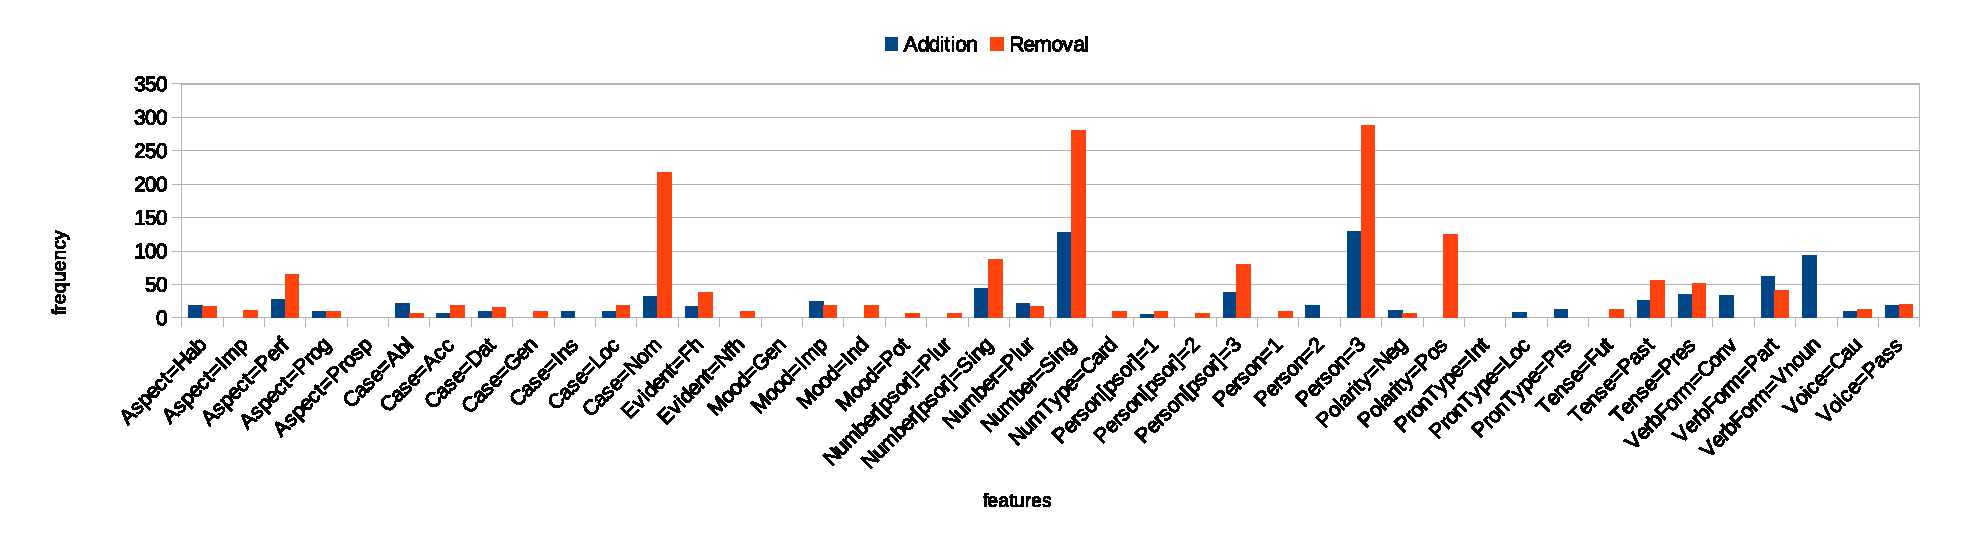
\includegraphics[width=0.99\linewidth]{figures/performance-incrase.eps}}
        \caption{The addition or removal of the features that improved the recovery.}
        \label{fig:subfig1}
    \end{subfigure}%
    
    \begin{subfigure}{0.9\textwidth}
        \centering
        \fbox{\includegraphics[width=1.1\linewidth]{figures/performance-decrease.eps}}
        \caption{The addition or removal of the features that reduced the recovery.}
        \label{fig:subfig2}
    \end{subfigure}
    \caption{\label{fig:impactoffeatureadditionandremoval} The impact of the addition and removal of features on the accuracy. }
\end{figure*}

\begin{table}
\centering
\begin{tabular}{|l|c|c|}
\hline
\multicolumn{1}{{|c|}}{\textbf{Model}} & \multicolumn{1}{{c|}}{\textbf{v2.8}} & \multicolumn{1}{{c|}}{\textbf{v2.11}} \\ \hline
GPT-3.5-Turbo       & 83.58          & 84.52    \\ \hline
Claude-instant-100k & 85.95          & 87.36    \\ \hline
GPT-4               & 89.97          & 91.28    \\ \hline
Claude-2-100k       & 89.00          & 90.53    \\ \hline
\hline 
& \multicolumn{2}{c|}{\textbf{UD\_English-EWT}}  \\ \hline
GPT-4              & \multicolumn{2}{c|}{94.00}  \\ \hline
\end{tabular}
\caption{The accuracy by sequence matching scores of the experiments with various large language models provided for \bounvOLD\ and \bounvNEW. The result for \ewt\ is provided for reference.}
\label{tab:results}
\end{table}


Several experiments using different large language models were conducted to compare alternative annotations of the same treebank. 
Specifically, the GPT-3.5, GPT-4~\cite{openai}, Claude Instant, and Claude 2~\cite{claude} models were prompted using the Poe API~\cite{poe}.

The proposed method was implemented with 500 randomly selected sentences that are consistent with the distribution of the number of tokens per sentence in the treebanks. 
A prompt was generated  for each annotated version of these sentences as explained in Section~\ref{sec:method}.
API calls were made to the above-mentioned models with these prompts and their responses were processed. 
Table~\ref{tab:results} shows the accuracy by sequence matching for both models.
Across all experiments, we observe a consistent increase of approximately 1.5\% in accuracy for \bounvNEW. 
This suggests that its annotations better capture the features of the sentences.

We also experimented with a treebank of another language, the \ewt\ treebank, to validate the method.
As GPT-4 produced the best results, we used only this model for this experiment.
The table shows that the model yields better recovery than all the models used for Turkish.
This may be regarded as an expected result since the GPT-4 model better captures the English language, and English sentences are somewhat easier to recover as they do not possess complex morphological features such as    morphologically rich languages like Turkish do.

Figure~\ref{fig:impactoffeatureadditionandremoval} illustrates the impact of adding and removing features during the re-annotation phase.
The most substantial improvement, attributed to the unique morphological feature tag and value, was achieved by removing the third-person annotation (i.e., Person=3) from a single token in the treebank during the transition from v2.8 to v2.11.
This change aided in producing the correct token 288 times, while it also led to the model producing an incorrect token 189 times.
The fact that the same feature tag and value pair (the third-person annotation) resulted  in both the most significant improvement and worsening of the performance underscores its significance in token recovery.
In Turkish, the third person is represented by two exponents: a null morpheme for singular and \textit{-lAr} for plural.
The fact that, as discussed in the previous sections, addressing a significant issue in Turkish that the UD framework has overlooked has had a notable impact on token recovery underscores the necessity to reconsider certain preconceptions and assumptions made by the UD framework regarding null morphemes.

While the removal of case and number can reduce accuracy in certain instances, it generally enhances overall performance. This suggests that the v2.8 version of the treebank may have had some level of clutter. Furthermore, the consistent improvement in annotation precision is observed when new features are added. It is essential to note that the addition of new features should be undertaken judiciously to prevent clutter and the annotation of non-existing layers of meaning.

To gain insight into the impact of annotations on recovering the surface forms of the sentences, various failures have been examined.
The reported accuracy scores are based on sequence matching over the entire sentence.
To gain a better understanding of the parts of the sentences that were not recovered accurately, the words within the sentences are examined along with their annotations.
By doing so, we aimed to understand the impact of the annotations in this task.
Since Turkish is a morphologically rich agglutinative language, the recoveries of the suffixes and their ordering are highly significant.

The percentage of produced tokens that matched the tokens and their order in the original sentences via prompting the GPT-4 model with the annotations from \bounvOLD\ and v2.11 are 73.7\%  and 75.4\% respectively (total number of tokens is \num{6247}).
The frequencies of the top five features for the words that were not  accurately recovered are shown in Table~\ref{tab:word-error-feature-analysis}. 

Except for polarity, these features belong to the nominal domain of Turkish, which is characterized by a high degree of syncretism. For example, the third-person possessive marker, \textit{-ı}, shares the same form as the accusative marker, \textit{-ı}. Consequently, this is an area where language models or parsers not engaged in syntax may struggle, as seen in v2.8. However, this confusion appears to have been minimized in v2.11. 

Additionally, the impact of  modifying the values of features was examined.
Table~\ref{tab:featurechange} shows the frequencies of improvement and worsening recovery for the most frequently used feature tags.

\begin{table}[tbh!]
\centering
\begin{tabular}{|l|S[table-format=4] | l | S[table-format=4] | l|}
\hline
\multicolumn{1}{|c|}{\textbf{Feature}} & \multicolumn{2}{c|}{\textbf{v2.8}} &  \multicolumn{2}{c|}{\textbf{v2.11}} \\ \cline{2-5} 
 & \multicolumn{1}{c|}{\textbf{\#}} & \multicolumn{1}{c|}{\textbf{\%}} & \multicolumn{1}{c|}{\textbf{\#}} & \multicolumn{1}{c|}{\textbf{\%}} \\ \hline
Person=3 & 1185 & 37 & 1167 &  35 \\ \hline
Number=Sing & 1072 & 36 & 1054 & 35 \\ \hline
Polarity=Pos & 459 & 49 & 570 & 51 \\ \hline
Case=Nom & 590 & 36 & 455 &  31 \\ \hline
Person[psor]=3 & 335 & 43 & 361 & 44 \\ \hline
\end{tabular}
\caption{The top 5 features of the words that were not accurately recovered for \bounvOLD\ and \bounvNEW, using GPT-4. }
\label{tab:word-error-feature-analysis}
\end{table}


\begin{table}[h]
\centering
\begin{tabular}{|l|c|c|S[table-format=2]|S[table-format=2]|}
\hline
\multicolumn{1}{|l|}{\textbf{Feature}} & \multicolumn{1}{c|}{\textbf{Old}} & \multicolumn{1}{c|}{\textbf{New}} & \multicolumn{1}{c|}{\textbf{+}} & \multicolumn{1}{c|}{\textbf{-}} \\[-2mm]
 & \multicolumn{1}{c|}{\textbf{Value}} & \multicolumn{1}{c|}{\textbf{Value}} & &  \\ \hline
Aspect & Hab & Perf & \textbf{--} & 12 \\ \hline
Aspect & Imp & Prog & \textbf{--} & 61 \\ \hline
Aspect & Imp & Prosp & 17 & \textbf{--} \\ \hline
Aspect & Prog & Imp & 33 & \textbf{--} \\ \hline
Aspect & Prosp & Imp & \textbf{--} & 11 \\ \hline
Case & Acc & Nom & \textbf{--} & 66 \\ \hline
Case & Dat & Nom & 11 & 9 \\ \hline
Case & Gen & Nom & 5 & \textbf{--} \\ \hline
Case & Loc & Nom & \textbf{--} & 6 \\ \hline
Case & Nom & Acc & 58 & \textbf{--} \\ \hline
Case & Nom & Dat & 6 & \textbf{--} \\ \hline
Case & Nom & Loc & 5 & \textbf{--} \\ \hline
Number & Plur & Sing & 16 & 12 \\ \hline
Number & Sing & Plur & 12 & 12 \\ \hline
Person & 3 & 1 & \textbf{--} & 5 \\ \hline
Person & 3 & 2 & \textbf{--} & 6 \\ \hline
\end{tabular}
\caption{\label{tab:featurechange} The impact of modifying the value of an existing feature. The  columns '+' and '-' show the frequencies for the increase and decrease in recovery.}
\end{table}

\section{Conclusions}
\label{sec:conclusions}
In this work, we examine the utility of large language models in evaluating the quality of corpora. The proposed approach was employed to examine the re-annotation  of a large Turkish treebank in the Universal Dependencies framework with a focus on linguistic improvements. For this purpose, we compared the annotations in the two different versions of the treebank.

Several LLM models were examined with prompts generated from the annotations of the two treebank versions to reconstruct the original sentences' surface forms. We observed, as expected, that LLMs that aim to capture linguistic characteristics provide useful information about the annotated treebanks and the annotation scheme. All models suggest an improvement regarding the re-annotation, with GPT-4 demonstrating the best performance. These results provide insights regarding the treebanks and the annotation scheme.

As future work, we plan to apply the proposed LLM-based evaluation scheme to other types of NLP resources. We believe that LLMs will be valuable in evaluating and gaining insight into language resources. This approach will contribute to creating higher-quality resources.

\nocite{*}
\section{Bibliographical References}\label{sec:reference}

\bibliographystyle{lrec-coling2024-natbib}
\bibliography{main}

\section{Language Resource References}
\label{lr:ref}
\bibliographystylelanguageresource{lrec-coling2024-natbib}
\bibliographylanguageresource{languageresource}


\end{document}


